\documentclass[11pt, oneside]{article}   	% use "amsart" instead of "article" for AMSLaTeX format


% \usepackage{draftwatermark}
% \SetWatermarkText{Draft}
% \SetWatermarkScale{5}
% \SetWatermarkLightness {0.9} 
% \SetWatermarkColor[rgb]{0.7,0,0}


\usepackage{geometry}                		% See geometry.pdf to learn the layout options. There are lots.
\geometry{letterpaper}                   		% ... or a4paper or a5paper or ... 
%\geometry{landscape}                		% Activate for for rotated page geometryhttps://www.washingtonpost.com/world/europe/amid-impeachment-probe-gordon-sondland-is-overseeing-a-renovation-of-his-residence-that-has-cost-1-million-in-taxpayer-money/2019/10/16/d0eece92-ef86-11e9-bb7e-d2026ee0c199_story.html?tid=sm_tw
%\usepackage[parfill]{parskip}    		% Activate to begin paragraphs with an empty line rather than an indent
\usepackage{graphicx}				% Use pdf, png, jpg, or eps� with pdflatex; use eps in DVI mode
								% TeX will automatically convert eps --> pdf in pdflat						\label{thm:integral_domain}

								% TeX will automatically convert eps --> pdf in pdflatex		
\usepackage{amssymb}
\usepackage{amsmath}
\usepackage{amsthm}
\usepackage{mathrsfs}
\usepackage[hyphens,spaces,obeyspaces]{url}
\usepackage{url}
\usepackage{hyperref}
\usepackage{subcaption}
\usepackage{authblk}
\usepackage{mathtools}
\usepackage{graphicx}
\usepackage[export]{adjustbox}
\usepackage{fixltx2e}
\usepackage{hyperref}
\usepackage{alltt}
\usepackage{color}
\usepackage[utf8]{inputenc}
\usepackage[english]{babel}
\usepackage{float}
\usepackage{bigints}
\usepackage{braket}
\usepackage{siunitx}
\usepackage{mathtools}



\usepackage[hyphenbreaks]{breakurl}

\newtheorem{thm}{Theorem}[section]
% \newtheorem{defn}[thm]{Definition}
\theoremstyle{definition}
\newtheorem{definition}{Definition}[section]
\newtheorem{proposition}{Proposition}[section]
\newtheorem{lemma}{Lemma}[section]
\newtheorem{example}{Example}[section]




\newcommand{\veq}{\mathrel{\rotatebox{90}{$=$}}}
\DeclareMathOperator{\bda}{\Big \downarrow}


\DeclareMathOperator{\E}{\mathbb{E}}
\newcommand{\argmax}{\operatornamewithlimits{argmax}}
\newcommand{\argmin}{\operatornamewithlimits{argmin}}

\title{CAP Rate vs. Cash Flow: What's The Difference?}
\author{David Meyer \\ dmm@\{1-4-5.net,uoregon.edu\}}

\date{Last update: \today}							% Activate to display a given date or no date



\begin{document}
\maketitle

\section{Introduction: CAP Rate}
When we read Commercial Real Estate (CRE) listings we are usually given the price, the Capitalization Rate (CAP Rate \cite{wiki:cap_rate}) and sometimes 
the Annual Net Operating Income (NOI \cite{wiki:noi}). 

\bigskip
\noindent
For example, in the Albertson's listing shown in Figure \ref{fig:albertsons} we are given the price (\$6,435,000.00) 
and the CAP Rate (6.0\%) but not the NOI. The CAP Rate is calculated as follows:\footnote{Note that some investors may calculate the cap rate differently.}

\bigskip
\begin{figure}[H]
\center{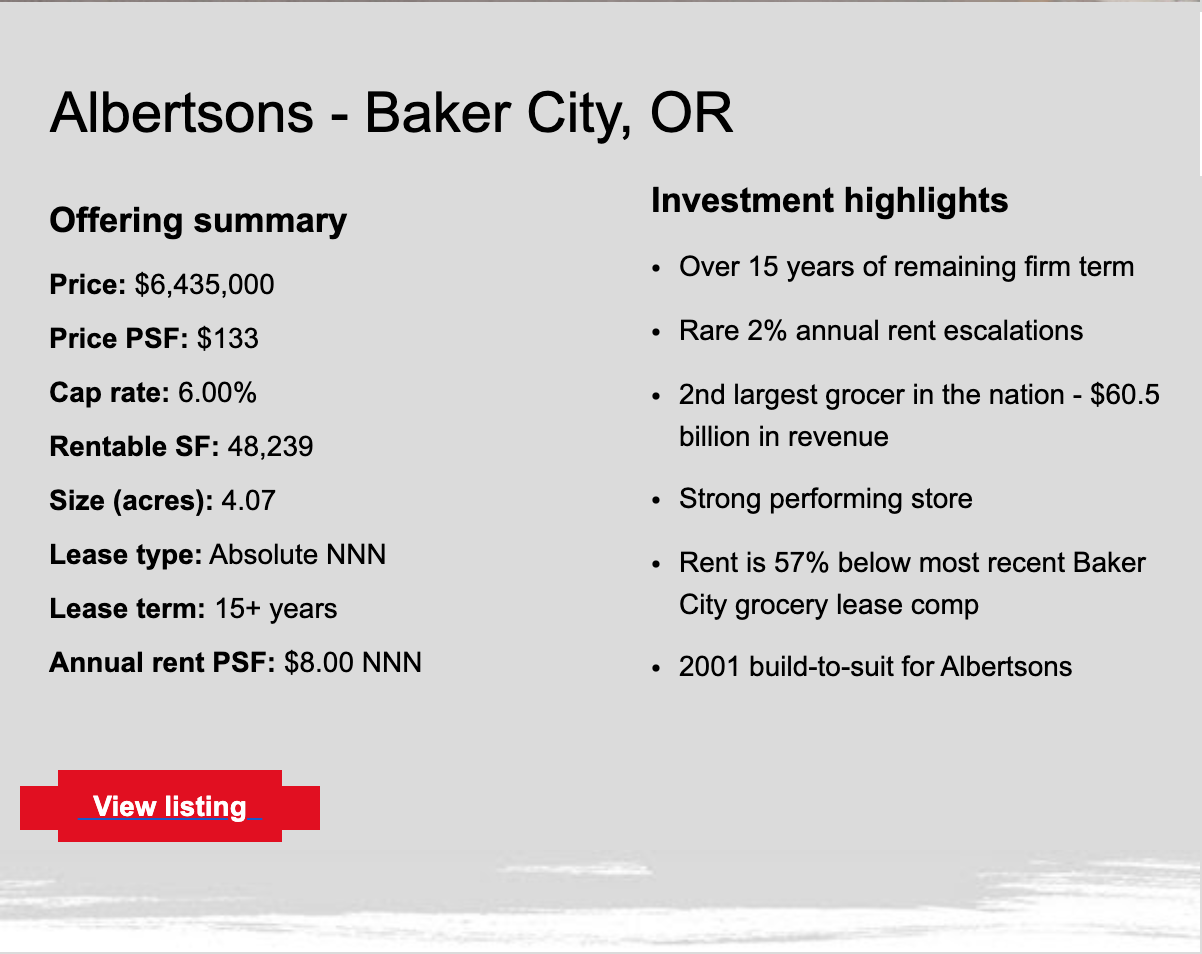
\includegraphics[scale=0.44, frame] {images/albertsons.png}}
\caption{Albertsons Baker City, OR Listing}
\label{fig:albertsons}
\end{figure}


\begin{equation*}
\text {Capitalization Rate} = \frac {\text{Annual net operating income}} {\text{Cost (or value)}}
\end{equation*}
 
 \bigskip
 \noindent
 or 
 
\begin{equation*}
\text {CAP Rate} = \frac {\text {NOI}} {\text{Cost}}
\end{equation*}

 

\bigskip
\noindent
For the Albertson's example, since we are given the Cost and the CAP rate, we can calculate the NOI:

\begin{equation*}
\text{NOI} = \text {CAP Rate} \times \text{Cost} = 0.06 \times \$6,435,000.00 = \$386,100.00
\end{equation*}

\bigskip
\noindent
But now the question is: \textbf{How is the NOI computed}?

\begin{itemize}
\item NOI = Net income - Operating Expenses
\begin{itemize}
\item Net Income (usually) consists of the rent we receive.
\item Importantly, \textbf{depreciation and mortgage payments} (both interest and principal) are not considered to be operating expenses and so \textbf{are not considered
to be part of the NOI}.
\end{itemize}
\item Cash Flow = NOI - Debt service
\begin{itemize}
\item Debt Service includes mortgage principal and interest payments.
\item Cash Flow is the money we will actually see.
\end{itemize}
\end{itemize}

\bigskip
\noindent
Luckily, there is a metric that we can use to look at Cash Flow (what we are concerned about in the near term): The Cash-on-Cash Return \cite{wiki:cash_on_cash}.

\section{Cash-on-Cash Return}
In investing, the \emph{cash-on-cash return} is the ratio of annual before-tax cash flow to the total amount of cash invested, expressed as a percentage.

\bigskip
\begin{equation*}
\text{cash-on-cash return} = \frac {\text{annual before-tax cash flow}}{\text{total cash invested}}
\end{equation*}

\bigskip
\noindent
or
\begin{equation}
\text{cash-on-cash return} =  \frac {\text{NOI - Debt Service}}{\text{total cash invested}}
\label{eqn:c-on-c}
\end{equation}

\bigskip
\noindent
The cash-on-cash return  is often used to evaluate the cash flow from income-producing assets. Generally considered a quick napkin test to determine if the asset qualifies for further review and analysis. Cash on Cash analyses are generally used by investors looking for properties where cash flow is paramount (such as in our case), however, some use it to determine if a property is undervalued, indicating instant equity in a property.

\subsection{Example}
Suppose we purchased a \$1,200,000 apartment complex with a \$300,000 down payment. Further, suppose that for each month, the cash flow from rentals, less expenses, is 
\$5,000. Then the annual before-tax income (NOI) would be $\$5,000 \times 12 = \$60,000$, so the NOI-on-cash return would be

\begin{equation*}
\frac {\$60,000}{\$300,000} = 0.20 = 20\%
\end{equation*}

\bigskip
\noindent
This gives us a bit better idea of the return on our investment (\$300,000). However, because we will have used debt to acquire some portion of the asset (the
property), we are required to make debt service payments (that is, mortgage payments).

\bigskip
\noindent
Because of this debt service the cash-on-cash 
return will be less than the CAP Rate, since the cash-on-cash return is computed by dividing the NOI minus all  mortgage payments by the total 
cash invested (see Equation \ref{eqn:c-on-c}).

\bigskip
\noindent
For example: If we had made total mortgage payments (principal+interest) of \$2,000 a month then the Debt Service and hence Cash Flow in this example would be: 

\begin{itemize}
\item Debt Service:  $\$2,000 \times 12 =  \$24,000$
\item Cash Flow:      $\text{NOI} - \text{Debt Service} = \$60,000 - \$24,000 = \$36,000$
\end{itemize}

\bigskip
\noindent
So the cash-on-cash return in this case would be

\begin{equation*}
\frac {\$36,000}{\$300,000} = 0.12 = 12\%
\end{equation*}

\bigskip
\noindent
Here the difference (20\% vs. 12\%) is accounted for by the required debt service. 

\bigskip
\noindent
This example also shows why it is much better to own these properties outright:
in that case $\textbf{Cash Flow}  \boldsymbol{=}  \textbf{NOI}$.

\subsection{A Few Limitations of cash-on-cash return}

\begin{itemize}
\item Because the calculation is based solely on before-tax cash flow relative to the amount of cash invested, it cannot take into account an individual investor's tax situation (much less eight of them) the particulars of which may influence the desirability of the investment. However an investor can usually deduct enough Capital Cost Allowance to defer the taxes for some period of time.

\item The formula does not take into account any appreciation or depreciation. When some cash is a return of capital (ROC) it will falsely indicate a higher return because ROC is not income.

\item cash-on-cash return does not account for other risks associated with the underlying property.

\item Finally, notice that cash-on-cash return is essentially a simple interest calculation and so ignores the effect of compounding interest. The implication for investors is that an 
investment with a lower nominal rate of compound interest may be superior in the long run to an investment with a higher cash-on-cash return.
\end{itemize}

\bigskip
\noindent
BTW, it is possible to perform an after-tax cash-on-cash calculation, but that would depend on an accurate estimate of our adjusted taxable income to correctly address how much tax payment is being saved through depreciation and other losses.


\bibliographystyle{ieeetr}
\bibliography{/Users/dmm/papers/finance/bib/finance}


\end{document} 
